\documentclass{article}

% Packages
\usepackage{amsmath}
\usepackage{amsfonts}
\usepackage{amssymb}
\usepackage{geometry}
\usepackage{tikz}
\usepackage{float}
\usepackage{enumitem}
\usepackage{mathtools}
\usepackage{subcaption}
\usepackage[colorlinks=true]{hyperref}
\usepackage{forest}


\forestset{
dg edges/.style={for tree={parent anchor=south, child anchor=north,align=center,base=bottom,where n children=0{tier=word,edge=dotted,calign with current edge}{}}},
}
% \usetikzlibrary{automata, arrows.meta, positioning,shapes}

\numberwithin{equation}{subsection}
\renewcommand{\thesubsection}{\thesection.\arabic{subsection}}
% \renewcommand{\thesubsubsection}{\Alph{subsubsection}}

\newcommand{\setsubsubsectionnumber}[1]{\setcounter{subsubsection}{#1}\addtocounter{subsubsection}{-1}}

\DeclareMathOperator{\putx}{put}

\makeatletter
\newcommand{\leqnomode}{\tagsleft@true}
\newcommand{\reqnomode}{\tagsleft@false}
\makeatother

\newcommand{\abs}[1]{\vert #1\vert}
\newcommand{\tab}[1][30pt]{\hspace*{#1}}
\newcommand{\bracket}[1]{\biggl[#1\biggr]}



\title{Theory of Machines and Languages - Assignment 3}
\author{Ali Abbasi - 98105879}
\begin{document}
\maketitle
\tableofcontents
\pagebreak

\section{Context Free Grammars}
\subsection{}
\subsubsection{}
A grammar describing the language is as follows:
\begin{align*}
S &\rightarrow bS \mid aA\\
A &\rightarrow bA \mid aB\\
B &\rightarrow bB \mid aC\\
C &\rightarrow bC \mid aC \mid \epsilon
\end{align*}

\subsubsection{}
\begin{align*}
S &\rightarrow ASA \mid 0\\
A &\rightarrow 0 \mid 1
\end{align*}

\subsection{}
We can rewrite the language as follows:
\begin{gather}
L=\left\{a^ib^jc^k \mid i, j, k \ge 0, i=j\right\} \cup 
\left\{a^ib^jc^k \mid i, j, k \ge 0, j=k\right\}
\end{gather}
So we have:
\begin{align*}
S &\rightarrow S_1 \mid S_2\\
S_1 &\rightarrow XC\\
C &\rightarrow cC \mid \epsilon\\
X &\rightarrow a X b \mid \epsilon\\
S_2 &\rightarrow AY\\
A &\rightarrow aA \mid \epsilon\\
Y &\rightarrow bYc \mid \epsilon
\end{align*}
Now consider the empty string (\(\epsilon\)).
Since in this string \(i=j\) and \(j=k\) both hold, it can be derived with both rules \(S\rightarrow S_1\) and \(S\rightarrow S_2\).
So this grammar is ambiguous.

\subsection{}
\subsubsection{}
Rightmost derivation of \(bbab\):
\begin{gather}
S \Rightarrow ST \Rightarrow Sb \Rightarrow TSb \Rightarrow TTSb \Rightarrow TTab \Rightarrow Tbab \Rightarrow bbab
\end{gather}
So the derivation tree is:
\begin{figure}[H]
    \centering
    \begin{forest}
        dg edges
        [S
            [S
                [T [b]]
                [S
                    [T [b]]
                    [S [a]]]]
            [T [b]]]
        \end{forest}  
\caption{Rightmost derivation tree for \(bbab\)}  
\label{fig:derivation_tree1}
\end{figure}

\subsubsection{}
\begin{gather}
S \Rightarrow TS \Rightarrow bS \Rightarrow bTS \Rightarrow bbS\Rightarrow bbST \Rightarrow bbaT \Rightarrow bbab
\end{gather}
And the derivation tree is:
\begin{figure}[H]
\centering
\begin{forest}
dg edges
[S
    [T [b]]
    [S
        [T [b]]
        [S
            [S [a]]
            [T [b]]]]]
\end{forest}    
\caption{Leftmost derivation tree for \(bbab\)}
\end{figure}
\subsubsection{}
As we saw, the string \(bbab\) had two different derivation trees
(we can reach the tree in Fig.~\ref{fig:derivation_tree1} by using leftmost derivations too.
So this string has two leftmost derivations).
Hence, this grammar is ambiguous.
The reason behind this is that it has two choices in some steps to generate \(b\)s around the \(a\).
\subsubsection{}
We can convert it to a unambiguous grammar as follows:
\begin{align*}
S &\rightarrow TaT\\
T &\rightarrow bT \mid \epsilon
\end{align*}


\subsection{}
Add new start variable:
\begin{equation}
\begin{aligned}
S_0 &\rightarrow S\\
S &\rightarrow ASB\\
A &\rightarrow aASA \mid a \mid \epsilon\\
B &\rightarrow SbS \mid A \mid bb
\end{aligned}
\end{equation}
Remove \(A \rightarrow \epsilon\):
\begin{equation}
\begin{aligned}
    S_0 &\rightarrow S\\
    S &\rightarrow ASB \mid SB\\
    A &\rightarrow aASA \mid a \mid aSA \mid aAS \mid aS\\
    B &\rightarrow SbS \mid A \mid bb \mid \epsilon
    \end{aligned}
\end{equation}
Remove \(B \rightarrow \epsilon\):
\begin{equation}
\begin{aligned}
    S_0 &\rightarrow S\\
    S &\rightarrow ASB \mid SB \mid S \mid AS\\
    A &\rightarrow aASA \mid a \mid aSA \mid aAS \mid aS\\
    B &\rightarrow SbS \mid A \mid bb
    \end{aligned}
\end{equation}
Remove \(S \rightarrow S\), \(S_0 \rightarrow S\), and \(B \rightarrow A\):
\begin{equation}
\begin{aligned}
S_0 &\rightarrow ASB \mid SB \mid AS\\
S &\rightarrow ASB \mid SB \mid AS\\
A &\rightarrow aASA \mid a \mid aSA \mid aAS \mid aS\\
B &\rightarrow SbS \mid A \mid bb \mid aASA \mid a \mid aSA \mid aAS \mid aS
\end{aligned}
\end{equation}
And finally, we convert all the remaining rules into the proper form.
\begin{equation}
\begin{aligned}
S_0 &\rightarrow AX \mid SB \mid AS\\
X &\rightarrow SB\\
S &\rightarrow AX \mid SB \mid AS\\
A &\rightarrow UY \mid a \mid UZ \mid UW \mid US\\
U &\rightarrow a\\
Y &\rightarrow AZ\\
Z &\rightarrow SA\\
W &\rightarrow AS\\
B &\rightarrow SK \mid VV \mid UY \mid a \mid UZ \mid UW \mid US\\
K &\rightarrow VS\\
V &\rightarrow b
\end{aligned}
\end{equation}

\subsection{To Do}

\section{Closure Properties of Context-Free Languages}
\subsection{}
Suppose that \(L_1\) and \(L_2\) are two context-free languages.
So there are CFGs that describe these languages, e.g. \(G_1\) and \(G_2\).
Then we can create a CFG that describes the concatenation of these languages as follows:
\begin{align*}
G_1 &= (V_1, \Sigma, R_1, S_1)\\
G_2 &= (V_2, \Sigma, R_2, S_2)\\
\implies G_3 &= (V_1 \cup V_2 \cup \{S\}, \Sigma, R_1 \cup R_2 \cup \{S \rightarrow S_1S_2\}, S)
\end{align*}
And \(G_3\) describes the concatenation of \(L_1\) and \(L_2\).
So the concatenation of two context-free languages is also context-free.

\subsection{}
First we convert the grammar of \(L\) to the Chomsky normal form. Then we convert this grammar (\(G\)) to a new grammar that recognizes the language \(PREFIX(L)\), proving that \(PREFIX(L)\) is context-free.
\begin{align*}
G &= (V, \Sigma, R, S)\\
\implies G_2 &= (V_2, \Sigma, R_2, S_\epsilon)\\
\text{Where } V_2 &= V \cup \left[\bigcup_{A \in V} \{A_\epsilon\}\right]\\
R_2 &= R \cup \left[\bigcup_{A\rightarrow BC \in R} \{A_\epsilon \rightarrow BC_\epsilon, A_\epsilon \rightarrow B_\epsilon\}\right] \cup \left[\bigcup_{A \rightarrow a \in R} \{A_\epsilon \rightarrow a\}\right] \cup \left[\bigcup_{A \in V} \{A_\epsilon \rightarrow \epsilon\}\right]
\end{align*}
For each \(A\) in the variables, we add a new variable \(A_\epsilon\), where \(A_\epsilon\) is nullable.
Then for each rule \(A \rightarrow BC\), we add two new rules: \(A_\epsilon \rightarrow BC_\epsilon\) and \(A_\epsilon \rightarrow B_\epsilon\). 
And also for we copy all rules generating terminals (like \(A \rightarrow a\)) for the new variables too (\(A_\epsilon \rightarrow a\)).
And we set \(S_\epsilon\) to be the start variable.\\
This way, if you consider the leftmost derivation of any string in \(L\), if we start from \(S_\epsilon\) instead of \(S\), then at each step of the derivation there is a \(\epsilon\) variable at the end of the string, where we can end the derivation right there by using the epsilon rule of that variable to get one of the strings in \(PREFIX(L)\), or act as before and proceed further.

\section{Pushdown Automata}
\subsection{}
\subsubsection{}
\begin{figure}[H]
\centering
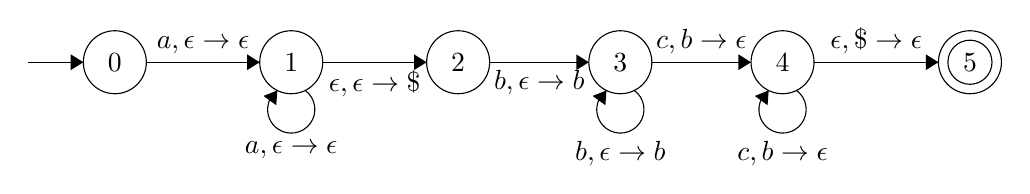
\begin{tikzpicture}[scale=0.2]
    \tikzstyle{every node}+=[inner sep=0pt]
    \draw [black] (5.7,-2.4) circle (2);
    \draw (5.7,-2.4) node {$0$};
    \draw [black] (16.9,-2.4) circle (2);
    \draw (16.9,-2.4) node {$1$};
    \draw [black] (37.8,-2.4) circle (2);
    \draw (37.8,-2.4) node {$3$};
    \draw [black] (48.1,-2.4) circle (2);
    \draw (48.1,-2.4) node {$4$};
    \draw [black] (60,-2.4) circle (2);
    \draw (60,-2.4) node {$5$};
    \draw [black] (60,-2.4) circle (1.4);
    \draw [black] (27.5,-2.4) circle (2);
    \draw (27.5,-2.4) node {$2$};
    \draw [black] (0.2,-2.4) -- (3.7,-2.4);
    \fill [black] (3.7,-2.4) -- (2.9,-1.9) -- (2.9,-2.9);
    \draw [black] (7.7,-2.4) -- (14.9,-2.4);
    \fill [black] (14.9,-2.4) -- (14.1,-1.9) -- (14.1,-2.9);
    \draw (11.3,-1.9) node [above] {$a,\epsilon\to\epsilon$};
    \draw [black] (39.8,-2.4) -- (46.1,-2.4);
    \fill [black] (46.1,-2.4) -- (45.3,-1.9) -- (45.3,-2.9);
    \draw (42.95,-1.9) node [above] {$c,b\to\epsilon$};
    \draw [black] (48.982,-4.186) arc (54:-234:1.5);
    \draw (48.1,-7.4) node [below] {$c,b\to\epsilon$};
    \fill [black] (47.22,-4.19) -- (46.34,-4.54) -- (47.15,-5.13);
    \draw [black] (50.1,-2.4) -- (58,-2.4);
    \fill [black] (58,-2.4) -- (57.2,-1.9) -- (57.2,-2.9);
    \draw (54.05,-1.9) node [above] {$\epsilon,\$\to\epsilon$};
    \draw [black] (38.682,-4.186) arc (54:-234:1.5);
    \draw (37.8,-7.4) node [below] {$b,\epsilon\to b$};
    \fill [black] (36.92,-4.19) -- (36.04,-4.54) -- (36.85,-5.13);
    \draw [black] (17.782,-4.186) arc (54:-234:1.5);
    \draw (16.9,-7.4) node [below] {$a,\epsilon\to\epsilon$};
    \fill [black] (16.02,-4.19) -- (15.14,-4.54) -- (15.95,-5.13);
    \draw [black] (18.9,-2.4) -- (25.5,-2.4);
    \fill [black] (25.5,-2.4) -- (24.7,-1.9) -- (24.7,-2.9);
    \draw (22.2,-2.9) node [below] {$\epsilon,\epsilon\to\$$};
    \draw [black] (29.5,-2.4) -- (35.8,-2.4);
    \fill [black] (35.8,-2.4) -- (35,-1.9) -- (35,-2.9);
    \draw (32.65,-2.9) node [below] {$b,\epsilon\to b$};
    \end{tikzpicture}
\caption{Pushdown automata for the language \(L=\left\{a^nb^mc^m\mid n, m \in \mathbb{N}\right\}\).}
\label{fig:automata3-1}
\end{figure}

\subsubsection{}
\begin{figure}[H]
\centering
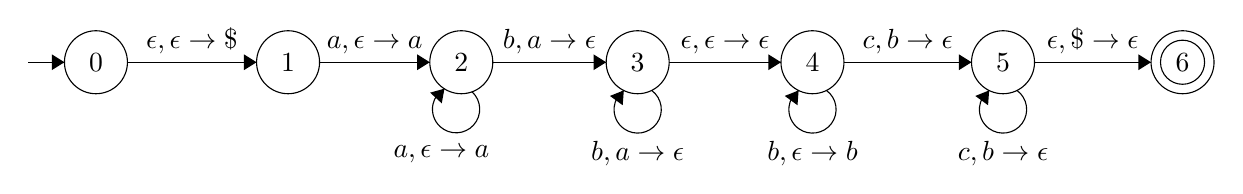
\begin{tikzpicture}[scale=0.2]
    \tikzstyle{every node}+=[inner sep=0pt]
    \draw [black] (27.7,-2.4) circle (2);
    \draw (27.7,-2.4) node {$2$};
    \draw [black] (38.9,-2.4) circle (2);
    \draw (38.9,-2.4) node {$3$};
    \draw [black] (50,-2.4) circle (2);
    \draw (50,-2.4) node {$4$};
    \draw [black] (62.1,-2.4) circle (2);
    \draw (62.1,-2.4) node {$5$};
    \draw [black] (73.5,-2.4) circle (2);
    \draw (73.5,-2.4) node {$6$};
    \draw [black] (73.5,-2.4) circle (1.4);
    \draw [black] (16.7,-2.4) circle (2);
    \draw (16.7,-2.4) node {$1$};
    \draw [black] (4.5,-2.4) circle (2);
    \draw (4.5,-2.4) node {$0$};
    \draw [black] (29.7,-2.4) -- (36.9,-2.4);
    \fill [black] (36.9,-2.4) -- (36.1,-1.9) -- (36.1,-2.9);
    \draw (33.3,-1.9) node [above] {$b,a\to \epsilon$};
    \draw [black] (28.379,-4.273) arc (47.65981:-240.34019:1.5);
    \draw (26.44,-7.66) node [below] {$a,\epsilon\to a$};
    \fill [black] (26.63,-4.08) -- (25.72,-4.33) -- (26.46,-5.01);
    \draw [black] (39.782,-4.186) arc (54:-234:1.5);
    \draw (38.9,-7.4) node [below] {$b,a\to \epsilon$};
    \fill [black] (38.02,-4.19) -- (37.14,-4.54) -- (37.95,-5.13);
    \draw [black] (40.9,-2.4) -- (48,-2.4);
    \fill [black] (48,-2.4) -- (47.2,-1.9) -- (47.2,-2.9);
    \draw (44.45,-1.9) node [above] {$\epsilon,\epsilon\to \epsilon$};
    \draw [black] (50.882,-4.186) arc (54:-234:1.5);
    \draw (50,-7.4) node [below] {$b,\epsilon\to b$};
    \fill [black] (49.12,-4.19) -- (48.24,-4.54) -- (49.05,-5.13);
    \draw [black] (52,-2.4) -- (60.1,-2.4);
    \fill [black] (60.1,-2.4) -- (59.3,-1.9) -- (59.3,-2.9);
    \draw (56.05,-1.9) node [above] {$c,b\to \epsilon$};
    \draw [black] (62.982,-4.186) arc (54:-234:1.5);
    \draw (62.1,-7.4) node [below] {$c,b\to \epsilon$};
    \fill [black] (61.22,-4.19) -- (60.34,-4.54) -- (61.15,-5.13);
    \draw [black] (64.1,-2.4) -- (71.5,-2.4);
    \fill [black] (71.5,-2.4) -- (70.7,-1.9) -- (70.7,-2.9);
    \draw (67.8,-1.9) node [above] {$\epsilon,\$\to \epsilon$};
    \draw [black] (18.7,-2.4) -- (25.7,-2.4);
    \fill [black] (25.7,-2.4) -- (24.9,-1.9) -- (24.9,-2.9);
    \draw (22.2,-1.9) node [above] {$a,\epsilon\to a$};
    \draw [black] (6.5,-2.4) -- (14.7,-2.4);
    \fill [black] (14.7,-2.4) -- (13.9,-1.9) -- (13.9,-2.9);
    \draw (10.6,-1.9) node [above] {$\epsilon,\epsilon\to\$$};
    \draw [black] (0.2,-2.4) -- (2.5,-2.4);
    \fill [black] (2.5,-2.4) -- (1.7,-1.9) -- (1.7,-2.9);
    \end{tikzpicture}
\caption{Pushdown automata for the language \(\left\{a^ib^jc^k\mid i,j,k\in \mathbb{N}, i+k=j\right\}\)}
\label{fig:automata3-1-2}
\end{figure}

\subsubsection{}
\begin{figure}[H]
\centering
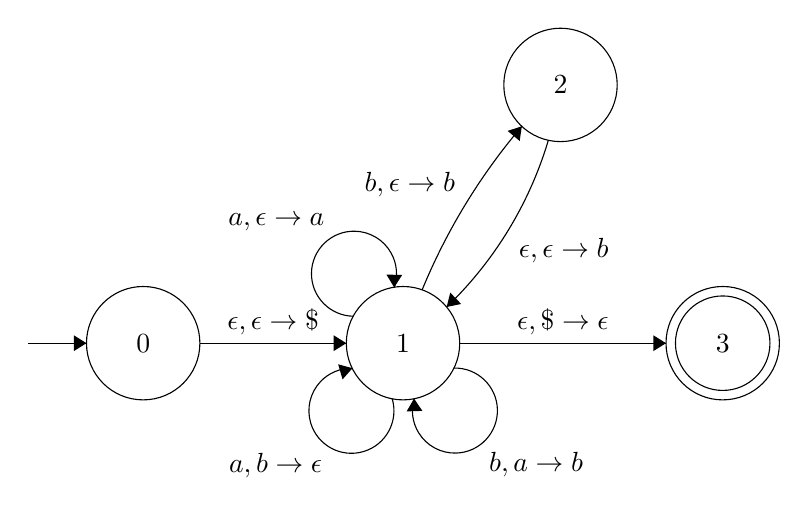
\begin{tikzpicture}[scale=0.2]
    \tikzstyle{every node}+=[inner sep=0pt]
    \draw [black] (7.5,-20.2) circle (3.6);
    \draw (7.5,-20.2) node {$0$};
    \draw [black] (24,-20.2) circle (3.6);
    \draw (24,-20.2) node {$1$};
    \draw [black] (34,-3.8) circle (3.6);
    \draw (34,-3.8) node {$2$};
    \draw [black] (44.3,-20.2) circle (3.6);
    \draw (44.3,-20.2) node {$3$};
    \draw [black] (44.3,-20.2) circle (3);
    \draw [black] (0.2,-20.2) -- (3.9,-20.2);
    \fill [black] (3.9,-20.2) -- (3.1,-19.7) -- (3.1,-20.7);
    \draw [black] (11.1,-20.2) -- (20.4,-20.2);
    \fill [black] (20.4,-20.2) -- (19.6,-19.7) -- (19.6,-20.7);
    \draw (15.75,-19.7) node [above] {$\epsilon,\epsilon\to\$$};
    \draw [black] (20.849,-18.488) arc (269.21759:-18.78241:2.7);
    \draw (15.96,-13.08) node [above] {$a,\epsilon\to a$};
    \fill [black] (23.44,-16.66) -- (23.95,-15.86) -- (22.95,-15.85);
    \draw [black] (23.31,-23.719) arc (16.64395:-271.35605:2.7);
    \draw (15.91,-27.13) node [below] {$a,b\to\epsilon$};
    \fill [black] (20.79,-21.79) -- (19.88,-21.54) -- (20.16,-22.5);
    \draw [black] (27.219,-21.78) arc (91.59101:-196.40899:2.7);
    \draw (32.45,-27.11) node [below] {$b,a\to b$};
    \fill [black] (24.7,-23.72) -- (24.23,-24.53) -- (25.23,-24.5);
    \draw [black] (25.214,-16.812) arc (157.63226:139.62173:38.842);
    \fill [black] (31.54,-6.43) -- (30.64,-6.72) -- (31.41,-7.36);
    \draw (27.33,-10.1) node [left] {$b,\epsilon\to b$};
    \draw [black] (33.228,-7.313) arc (-16.62882:-46.11719:24.373);
    \fill [black] (26.77,-17.9) -- (27.69,-17.71) -- (27,-16.99);
    \draw (31.32,-14.3) node [right] {$\epsilon,\epsilon\to b$};
    \draw [black] (27.6,-20.2) -- (40.7,-20.2);
    \fill [black] (40.7,-20.2) -- (39.9,-19.7) -- (39.9,-20.7);
    \draw (34.15,-19.7) node [above] {$\epsilon,\$\to\epsilon$};
    \end{tikzpicture}
\caption{Pushdown automata for the language \(\left\{w\in\{a,b\}^*\mid n_a(w)=2n_b(w)\right\}\)}
\label{fig:automata3-1-3}
\end{figure}
Reading each \(b\) either pushes two \(b\)s to the stack or pops an \(a\) and adds a \(b\) to the stack.
Reading each \(a\) either pushes and \(a\) to or pops a \(b\) from the stack.

\subsection{}
\begin{figure}[H]
\centering
    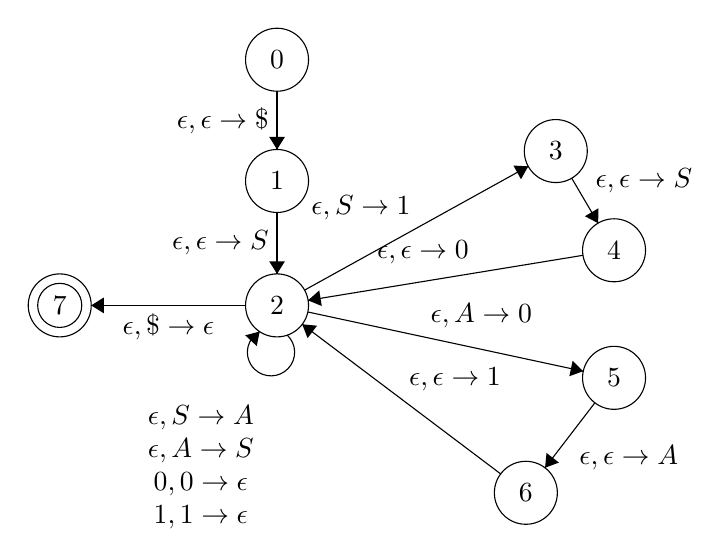
\begin{tikzpicture}[scale=0.2]
    \tikzstyle{every node}+=[inner sep=0pt]
    \draw [black] (19.2,-2.2) circle (2);
    \draw (19.2,-2.2) node {$0$};
    \draw [black] (19.2,-9.9) circle (2);
    \draw (19.2,-9.9) node {$1$};
    \draw [black] (19.2,-17.8) circle (2);
    \draw (19.2,-17.8) node {$2$};
    \draw [black] (36.9,-8) circle (2);
    \draw (36.9,-8) node {$3$};
    \draw [black] (40.6,-14.3) circle (2);
    \draw (40.6,-14.3) node {$4$};
    \draw [black] (40.6,-22.4) circle (2);
    \draw (40.6,-22.4) node {$5$};
    \draw [black] (35,-29.7) circle (2);
    \draw (35,-29.7) node {$6$};
    \draw [black] (5.4,-17.8) circle (2);
    \draw (5.4,-17.8) node {$7$};
    \draw [black] (5.4,-17.8) circle (1.4);
    \draw [black] (19.2,-4.2) -- (19.2,-7.9);
    \fill [black] (19.2,-7.9) -- (19.7,-7.1) -- (18.7,-7.1);
    \draw (18.7,-6.05) node [left] {$\epsilon,\epsilon\to\$$};
    \draw [black] (19.2,-11.9) -- (19.2,-15.8);
    \fill [black] (19.2,-15.8) -- (19.7,-15) -- (18.7,-15);
    \draw (18.7,-13.85) node [left] {$\epsilon,\epsilon\to S$};
    \draw [black] (20.95,-16.83) -- (35.15,-8.97);
    \fill [black] (35.15,-8.97) -- (34.21,-8.92) -- (34.69,-9.79);
    \draw (24.53,-12.39) node [above] {$\epsilon,S\to 1$};
    \draw [black] (37.91,-9.72) -- (39.59,-12.58);
    \fill [black] (39.59,-12.58) -- (39.61,-11.63) -- (38.75,-12.14);
    \draw (39.4,-9.9) node [right] {$\epsilon,\epsilon\to S$};
    \draw [black] (38.63,-14.62) -- (21.17,-17.48);
    \fill [black] (21.17,-17.48) -- (22.04,-17.84) -- (21.88,-16.85);
    \draw (28.46,-15.23) node [above] {$\epsilon,\epsilon\to 0$};
    \draw [black] (21.16,-18.22) -- (38.64,-21.98);
    \fill [black] (38.64,-21.98) -- (37.97,-21.32) -- (37.76,-22.3);
    \draw (32.17,-19.29) node [above] {$\epsilon,A\to 0$};
    \draw [black] (39.38,-23.99) -- (36.22,-28.11);
    \fill [black] (36.22,-28.11) -- (37.1,-27.78) -- (36.31,-27.17);
    \draw (38.37,-27.46) node [right] {$\epsilon,\epsilon\to A$};
    \draw [black] (33.4,-28.5) -- (20.8,-19);
    \fill [black] (20.8,-19) -- (21.14,-19.88) -- (21.74,-19.09);
    \draw (30.5,-23.25) node [above] {$\epsilon,\epsilon\to 1$};
    \draw [black] (19.846,-19.684) arc (46.66562:-241.33438:1.5);
    \draw (14.36,-24.1) node [below, align=center] {\(\epsilon,S\to A\)\\
    \(\epsilon,A\to S\)\\
    \(0,0\to \epsilon\)\\
    \(1,1\to \epsilon\)
    };
    \fill [black] (18.1,-19.46) -- (17.18,-19.7) -- (17.91,-20.38);
    \draw [black] (17.2,-17.8) -- (7.4,-17.8);
    \fill [black] (7.4,-17.8) -- (8.2,-18.3) -- (8.2,-17.3);
    \draw (12.3,-18.3) node [below] {$\epsilon,\$\to\epsilon$};
    \end{tikzpicture}
\caption{Pushdown automata for the grammar.}
\label{fig:automata3-2}
\end{figure}

\subsection{To Do}

\section{Pumping Lemma for Context-Free Languages}
\subsection{}
Suppose it holds.
Consider the language \(L=\left\{a^nb^mc^md^{3n}\mid m,n \ge 1\right\}\).
\(L\) is context-free, since there is a CFG describing it:
\begin{align*}
S &\to aSddd \mid aTddd\\
T &\to bTc \mid bc
\end{align*}
So \(L_{1/2}\) will be as follows:
\begin{align*}
L_{1/2}&=
\begin{cases}
a^nb^mc^n & m\ge n\\
a^nb^mc^md^{n-m} & m<n
\end{cases} & m,n\ge 1
\end{align*}
Suppose its pumping length is \(p\).
Let \(s=a^pb^pc^p\) and \(s\in L_{1/2}\).
As its length is more than \(p\), \(a^pb^pc^p\) must be pumped.
But we can show it cannot be pumped.
\begin{align*}
\exists u,v,x,y,z:
\begin{cases}
a^pb^pc^p = uvxyz&\\
uv^ixy^iz\in L_{1/2} & i\ge 0\\
\abs{vxy} \le p&\\
\abs{vy} > 0&
\end{cases}
\end{align*}
Consider two cases below:
\begin{itemize}
\item Either \(v\) or \(y\) contains more than one type of symbol, the order of symbols in \(uv^2xy^2z\) will not be in the correct order.
\item Both \(v\) and \(y\) have only one type of alphabet.
There can be 3 cases:
\begin{itemize}
\item \(v\) and \(y\) both contain only \(a\) or both contain only \(c\).
In this case, number of \(a\)s and \(c\)s in \(uv^2xy^2z\) will not be equal and it will not be in the language.
\item \(v\) and \(y\) both contain only \(b\).
In this case, \(uxz\) will have less \(b\)s than \(a\)s and \(c\)s.
Therefore it isn't a member of \(L_{1/2}\).
\item \(v\) contains \(a\) and \(y\) contains \(b\), or \(v\) contains \(b\) and \(y\) contains \(c\).
In this both of these cases, \(uv^2xy^2z\) will have different number of \(a\) and \(c\).
\end{itemize}
\end{itemize}
So we've shown that \(a^pb^pc^p\) cannot be pumped and reached a contradiction.
Thus the mentioned rule does not hold.

\subsection{}
We first assume these languages are context free, then we prove that they can't be pumped.
\subsubsection{}
\begin{align*}
L&=\left\{w\in \left\{a, b, c\right\}^*\mid n_a(w) < n_b(w) < n_c(w)\right\}
\end{align*}
Consider the string \(a^pb^{p+1}c^{p+2}\).
\begin{align*}
\exists u,v,x,y,z:
\begin{cases}
a^pb^{p+1}c^{p+2} = uvxyz&\\
uv^ixy^iz\in L & i\ge 0\\
\abs{vxy} \le p&\\
\abs{vy} > 0&
\end{cases}
\end{align*}
There are three cases for \(v\) and \(y\):
\begin{itemize}
\item Either \(v\) or \(y\) contains more than one type of symbol, the order of symbols in \(uv^2xy^2z\) will not be in the correct order.
\item Both \(v\) and \(y\) have only one type of alphabet and both contain the same symbol.
\begin{itemize}
\item If both contain only \(a\), then the number of \(a\) symbols in \(uv^2xy^2z\), will be greater than or equal to number of \(b\) symbols.
\item If both contain only \(b\), then the number of \(b\) symbols in \(uv^2xy^2z\), will be greater than or equal to number of \(c\) symbols.
\item If both contain only \(c\), then the number of \(c\) symbols in \(uxz\), will be less than or equal to number of \(b\) symbols.
\end{itemize}
\item Both \(v\) and \(y\) have only one type of alphabet and contain different symbols.
There can be two cases:
\begin{itemize}
\item \(v\) contains \(a\) and \(y\) contains \(b\).
\begin{itemize}
\item If \(y\) is not empty, then the number of \(b\) symbols in \(uv^2xy^2z\), will be greater than or equal to number of \(c\) symbols.
\item If \(y\) is empty, then the number of \(a\) symbols in \(uv^2xy^2z\), will be greater than or equal to number of \(b\) symbols.
\end{itemize}
\item \(v\) contains \(b\) and \(y\) contains \(c\).
\begin{itemize}
\item If \(v\) is not empty, then the number of \(b\) symbols in \(uxz\) will be less than or equal to number of \(a\) symbols.
\item If \(v\) is empty, then the number of \(c\) symbols in \(uxz\) will be less than or equal to number of \(b\) symbols.
\end{itemize}
\end{itemize}
\end{itemize}
So we've shown that \(a^pb^{p+1}c^{p+2}\) cannot be pumped and reached a contradiction.

\subsubsection{}
\begin{align*}
L=\left\{w\in \{a, b\}^* \mid w=w^R, n_a(w)=n_b(w)\right\} 
\end{align*}
Consider the string \(s=a^pb^{2p}a^{p}\).
\begin{align*}
\exists u,v,x,y,z:
\begin{cases}
a^pb^{2p}a^{p} = uvxyz&\\
uv^ixy^iz\in L & i\ge 0\\
\abs{vxy} \le p&\\
\abs{vy} > 0&
\end{cases}
\end{align*}
\begin{itemize}
\item If either \(v\) or \(y\) contains more than one type of symbol, the order of symbols in \(uv^2xy^2z\) will not be in the correct order.
\item Both \(v\) and \(y\) have only one type of alphabet and both contain the same symbol.
In this case \(uv^2xy^2z\), the number of \(a\) and \(b\)s will be different.
\item \(v\) contains \(a\) and \(y\) contains \(b\) or vice versa.
In this case, \(uv^2xy^2z\) will not be symmetric.
\end{itemize}
So we've shown that \(a^pb^{2p}a^{p}\) cannot be pumped and reached a contradiction.

\subsubsection{}
\begin{align*}
L=\left\{a^ib^j\mid i=kj \text{ for some positive integer } k\right\}
\end{align*}
Consider the string \(s=a^{2p^2}b^{2p}\).
As \(\abs{s}\) is greater than \(p\), it can be pumped:
\begin{align*}
\exists u,v,x,y,z:
\begin{cases}
a^{2p^2}b^{2p} = uvxyz&\\
uv^ixy^iz\in L & i\ge 0\\
\abs{vxy} \le p&\\
\abs{vy} > 0&
\end{cases}
\end{align*}
There are two cases for \(v\) and \(y\):
\begin{itemize}
\item Either \(v\) or \(y\) contains more than one type of symbol.
In this case, the order of symbols in \(uv^2xy^2z\) will not be in the correct order.
\item Both \(v\) and \(y\) have only one type of alphabet and both contain the same symbol.
\begin{itemize}
\item Both contain \(a\).
Suppose \(\abs{vy}=n\).
We have:
\begin{align*}
\forall i:\ &2p\mid 2p^2 + (i-1)n\\
\implies \forall i:\ &2p\mid (i-1)n\\
\implies &2p\mid n\\
\implies &n \ge 2p
\end{align*}
Which is a contradiction.
Because we know \(n=\abs{vy}\le \abs{vxy} \le  p\).
\item Both contain \(b\).
In this case we can find a \(i\) large enough such that \(uv^ixy^iz\) contains more \(b\)s than \(a\)s.
\item \(v\) contains \(a\) and \(y\) contains \(b\).
Assume \(\abs{v}=n\) and \(\abs{y}=m\). We have:
\begin{align*}
\forall i:\ &2p+(i-1)m\mid 2p^2 + (i-1)n\\
\implies \forall i:\ &2p+(i-1)m\mid (i-1) (n-pm)\\
\implies &n-pm = 0\\
\implies &n = pm\\
\implies &\abs{vy} = (p+1)m > p
\end{align*}
Which is again, a contradiction because we know \(\abs{vy} \le p\).
\end{itemize}
\end{itemize}
So we've shown that \(a^{2p^2}b^{2p}\) cannot be pumped and reached a contradiction.



\end{document}